\documentclass[a4paper, 12pt]{article}

\usepackage{graphicx} % Required for the inclusion of images
\usepackage{amsmath} % Required for some math elements 
\usepackage{times} % Uncomment to use the Times New Roman font

\title{Institute of Engineering,\\ Thapathali Campus \\ Computer Aided Drawing \\ ME 505} % Title
\author{Bibek Magar}
\date{\today} % Date for the report

\begin{document}
\maketitle % Insert the title, author and date
	\begin{center}
		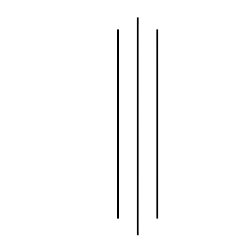
\includegraphics{gfx/lines.png}
	\end{center}
	\begin{center}
		\textbf{Lab manual for Computer Aided Drawing}
	\end{center}
	
	\newpage

\section{lab 1: Introduction to AutoCAD interface and coordinate systems}
\begin{center}
	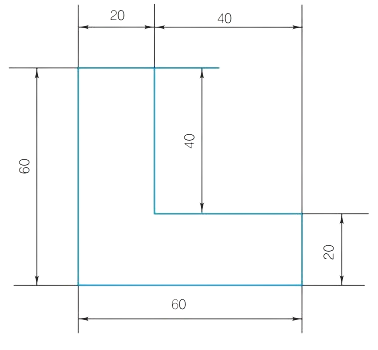
\includegraphics{gfx/fig.png}
\end{center}
\emph{Assume absolute coordinate of the bottom left corner be (15, 15).}
\subsection{Draw the given figure in AutoCAD using the absolute coordinates and write the command sequence.}
\subsection{Draw the given figure in AutoCAD using the relative coordinates and write the command sequence.}
\subsection{Draw the given figure in AutoCAD using the relative polar coordinates and write the command sequence.}
\clearpage
%lab2
\section{lab 2: Introduction to AutoCAD sketch tools}
\subsection{Draw a parabola with double ordinate 100 mm and axis 60 mm. }
\subsection{Draw the given figure in AutoCAD and write the command sequence.}
\begin{center}
    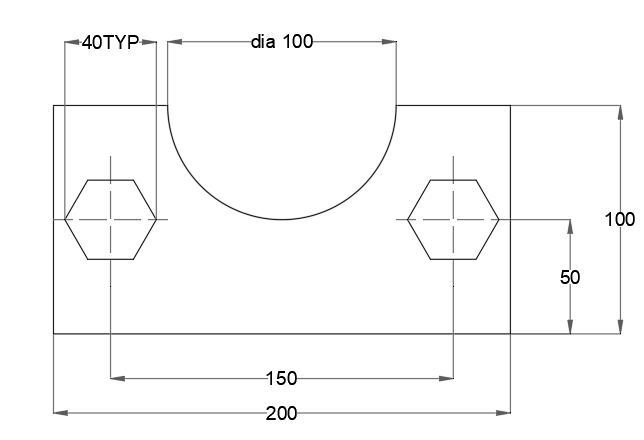
\includegraphics{gfx/l2t2.PNG}
\end{center}
\subsection{Draw the given figure in AutoCAD and write the command sequence.}
\begin{center}
    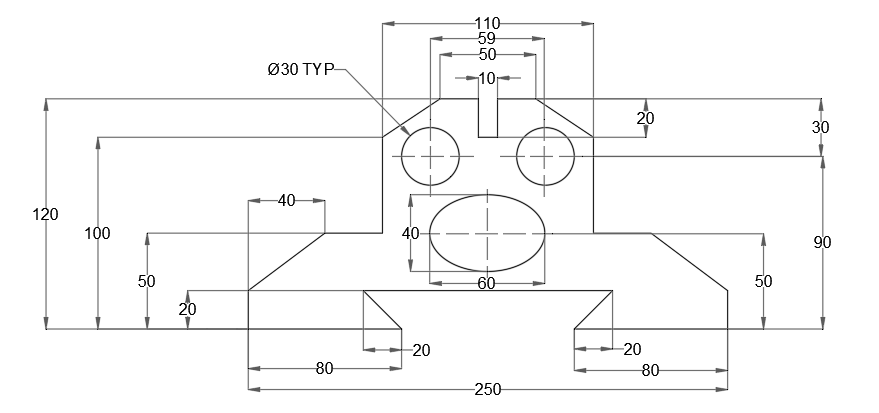
\includegraphics[scale = 0.7]{gfx/l2t3.PNG}
\end{center}
\end{document}